% \def\r{Pearson's r\xspace}
\def\ktau{Kendall's $\tau$\xspace}
\def\srho{Spearman's $\rho$\xspace}
\def\pb{Pointbiserial\xspace}
\def\student{Student's t-test\xspace}
\def\paired{Paired t-test\xspace}
\def\mannu{Mann-Whitney U\xspace}
\def\wilcox{Wilcoxon signed rank\xspace}
\def\welch{Welch's t-test\xspace}
\def\f{F-test\xspace}
\def\rm{Repeated measures one way ANOVA\xspace}
\def\kw{Kruskal Wallis\xspace}
\def\friedman{Friedman\xspace}
\def\facANOVA{Factorial ANOVA\xspace}
\def\twoANOVA{Two-way ANOVA\xspace}
\def\chiSq{Chi Square\xspace}
\def\fisher{Fisher's Exact\xspace}
\def\boot{Bootstrap\xspace}


\newcommand{\figureTeaProgram}{
\begin{figure}
    % \vspace{-5pt}
    \centering
    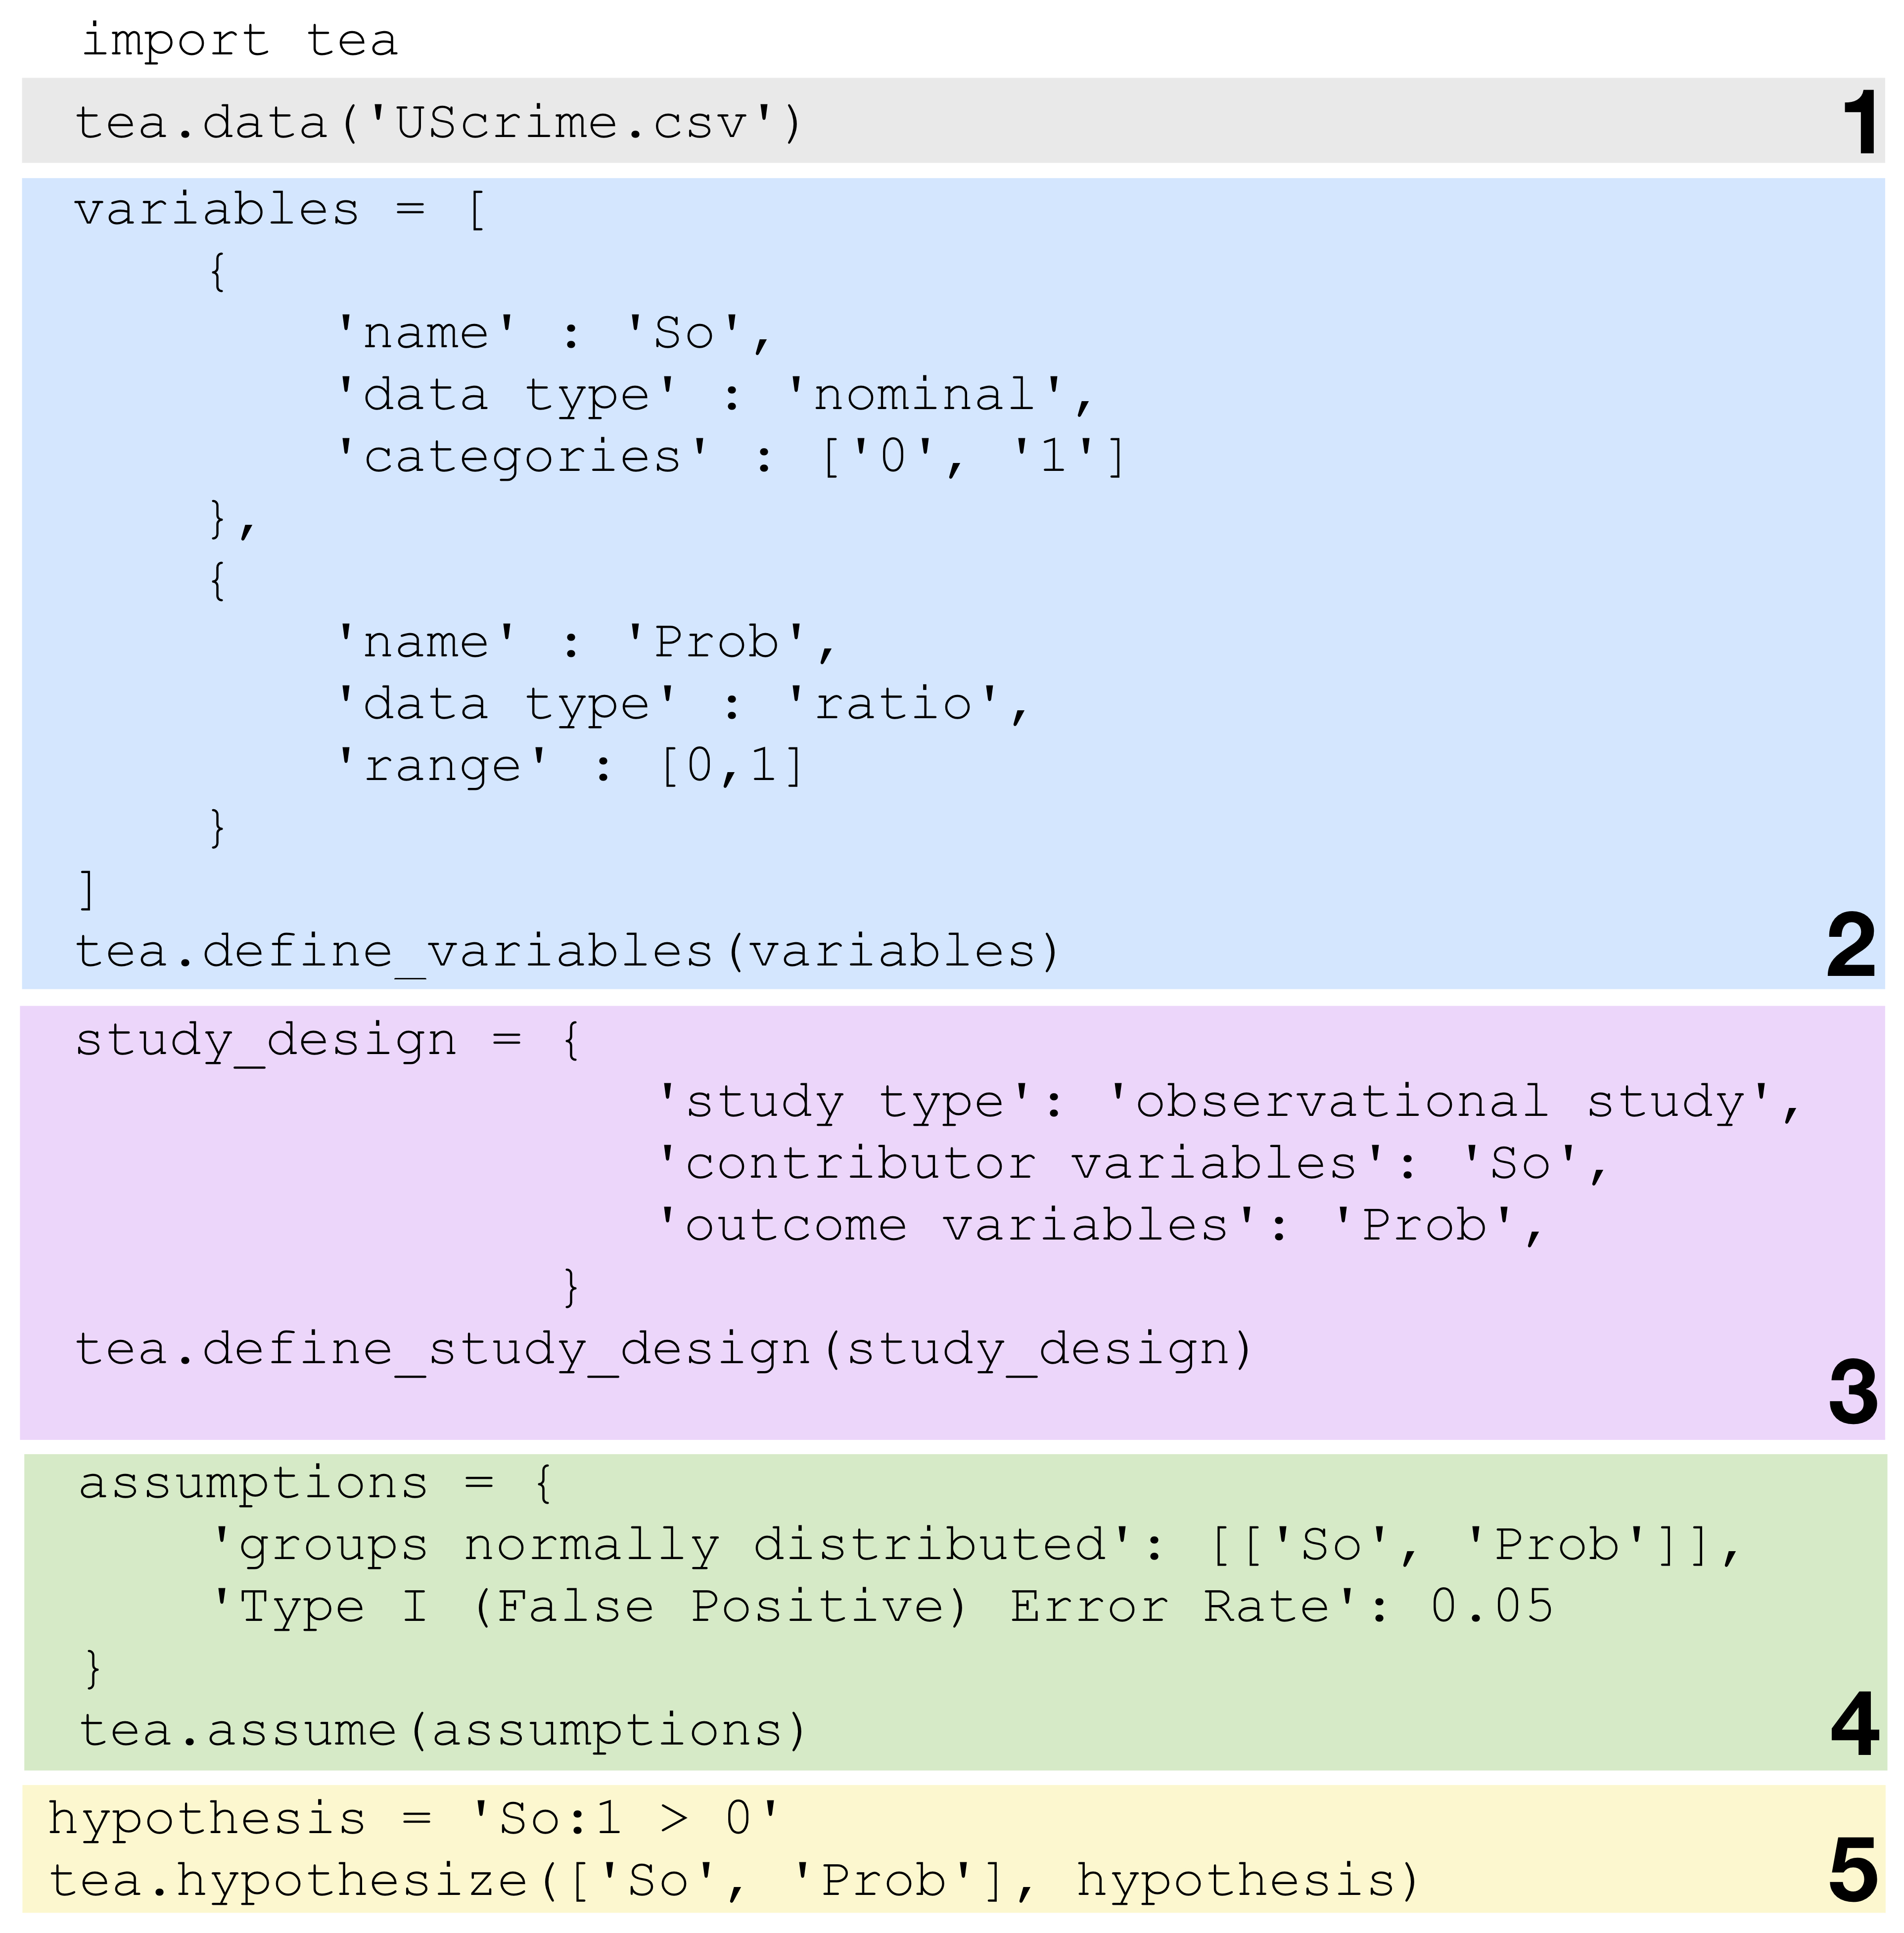
\includegraphics[width=0.5\columnwidth, clip]{tea/figures/tea_program.jpg}
    % \vspace{-15pt} 
    \caption{\textbf{Sample Tea program.} The specification outlines an experiment to analyze the relationship between geographic location (`So') and probability of imprisonment (`Prob') in a common USCrime data set~\protect\cite{venables2013modern,kabacoff2011action}.
    See~\autoref{usageScenarioTea} for an explanation of the code. Tea programs specify 1) data, 2) variables, 3) study design, 4) assumptions, and 5) hypotheses.}
    \label{fig:tea_program}
    \vspace{-\baselineskip}
\end{figure}
}


\def\r{Pearson's r}
\def\ktau{Kendall's $\tau$}
\def\srho{Spearman's $\rho$}
\def\pb{Pointbiserial}
\def\student{Student's t-test}
\def\paired{Paired t-test}
\def\mannu{Mann-Whitney U}
\def\wilcox{Wilcoxon signed rank}
\def\welch{Welch's}
\def\f{F-test}
\def\rm{Repeated measures one way ANOVA}
\def\kw{Kruskal Wallis}
\def\friedman{Friedman}
\def\facANOVA{Factorial ANOVA}
\def\twoANOVA{Two-way ANOVA}
\def\chiSq{Chi Square}
\def\fisher{Fisher's Exact}

\newcommand{\tableTeaTests}{
    \begin{table*}[htbp]
      \begin{center} \singlespacing
      \caption{Statistical tests supported in Tea's Null Hypothesis Significance Testing module} \label{tab:tea_tests}
      \begin{tabular}{lll}
      \toprule
      \colH{Class of tests}           & \colH{Parametric} & \colH{Non-parametric} \\
        Correlation                   & \r                &  \ktau   \\
                                      & \pb               &  \srho  \\
        \midrule
        Bivariate mean comparison     & \student          & \welch \\
                                      &                   & \mannu \\
                                      &                   & (a.k.a. Wilcoxon rank sum) \\
                                      & \paired           & \wilcox \\
        \midrule
        Multivariate mean comparison  & \f                & \kw   \\
                                      & \rm               & \friedman \\
                                      & \twoANOVA         & \\
                                      & \facANOVA         & \\
        \midrule
        \midrule
        Proportions: \chiSq , \fisher and Others: Bootstrapping (with confidence intervals) \\
      \bottomrule
      \end{tabular}
      \end{center}
    \end{table*}
}

\newcommand{\furtherTestResults}{
\begin{table*}[htbp]
  \begin{center}
    \caption{Results from Factorial ANOVA for RM ANOVA example.}
    \begin{tabularx}{\linewidth}{XXXXXX}
       & \textbf{df} & \textbf{sum\_sq} & \textbf{mean\_sq} & \textbf{F} & \textbf{PR(>F)} \\
      C(conc) & 6.0 & 4068.771429 & 678.128571 & 9.261087 & 1.242777e-07 \\
      Residual & 77.0 & 5638.204167  & 73.223431   &    NaN     &      NaN \\
    \end{tabularx}
    \end{center}
    \label{tab:rm_anova_fanova}
\end{table*}

\begin{table*}[htpb]
  \begin{center}
    \caption{Results from F test for F test example.}
    \begin{tabularx}{\linewidth}{XXXXXX}
       & \textbf{df} & \textbf{sum\_sq} & \textbf{mean\_sq} & \textbf{F} & \textbf{PR(>F)} \\
        C(trt)   &  4.0 & 1351.369014 & 337.842253 & 32.432826 & 9.818516e-13 \\
        Residual & 45.0 &  468.750438  & 10.416676    &    NaN       &    NaN \\
    \end{tabularx}
  \end{center}
  \label{tab:f_test_f_test}
\end{table*}

\begin{table*}[htpb]
  \begin{center}
    \caption{Results from Factorial ANOVA test for F test example.}
    \begin{tabularx}{\linewidth}{XXXXXX}
       & \textbf{df} & \textbf{sum\_sq} & \textbf{mean\_sq} & \textbf{F} & \textbf{PR(>F)} \\
        C(trt)   &  4.0 & 1351.369014 & 337.842253 & 32.432826 & 9.818516e-13 \\
        Residual & 45.0 &  468.750438  & 10.416676    &    NaN       &    NaN \\
    \end{tabularx}
  \end{center}
  \label{tab:f_test_fanova}
\end{table*}

\begin{table*}[htpb]
  \begin{center}
    \caption{Results from Factorial ANOVA test for Paired T test example.}
    \begin{tabularx}{\linewidth}{XXXXXX}
       & \textbf{df} & \textbf{sum\_sq} & \textbf{mean\_sq} & \textbf{F} & \textbf{PR(>F)} \\
        C(Group) &  1.0 &  294.0  &  294.0 & 2.826923 & 0.106839 \\
        Residual & 22.0 & 2288.0  &  104.0    &   NaN   &    NaN \\
    \end{tabularx}
  \end{center}
  \label{tab:paired_t_fanova}
\end{table*}


\begin{table*}[htpb]
  \begin{center}
    \caption{Results from F test and Factorial ANOVA for Student's T test example.}
    \begin{tabularx}{\linewidth}{XXXXXX}
       & \textbf{df} & \textbf{sum\_sq} & \textbf{mean\_sq} & \textbf{F} & \textbf{PR(>F)} \\
        C(So)   &   1.0 &  0.006702 &  0.006702 & 17.657903 & 0.000124 \\
        Residual & 45.0 & 0.017079 & 0.000380    &    NaN     &  NaN \\
    \end{tabularx}
  \end{center}
  \label{tab:students_t_f_test_and_fanova}
\end{table*}
}

% make a custom style that looks good and can highlight some additional keywords
\lstdefinestyle{tea}{
  basicstyle=\ttfamily,
  deletekeywords={input, print, id},
  language=Python,
  % here are the additional keywords
  emph={load_data, hypothesize, <, >, =, !},
  % they are underlines
  emphstyle={\bf},
}
\lstset{
  % use this style by default
  style=tea,
  % look better
  columns=flexible,
  showstringspaces=false,
  % spacing, size, numbers, etc.
  numbers=left,
  xleftmargin=2em,
  numberstyle=\tiny,
  escapechar=|,
}


\newcommand{\teaHypotheses}{
  \begin{figure}[t]
    \vspace{-5pt}
    \centering
    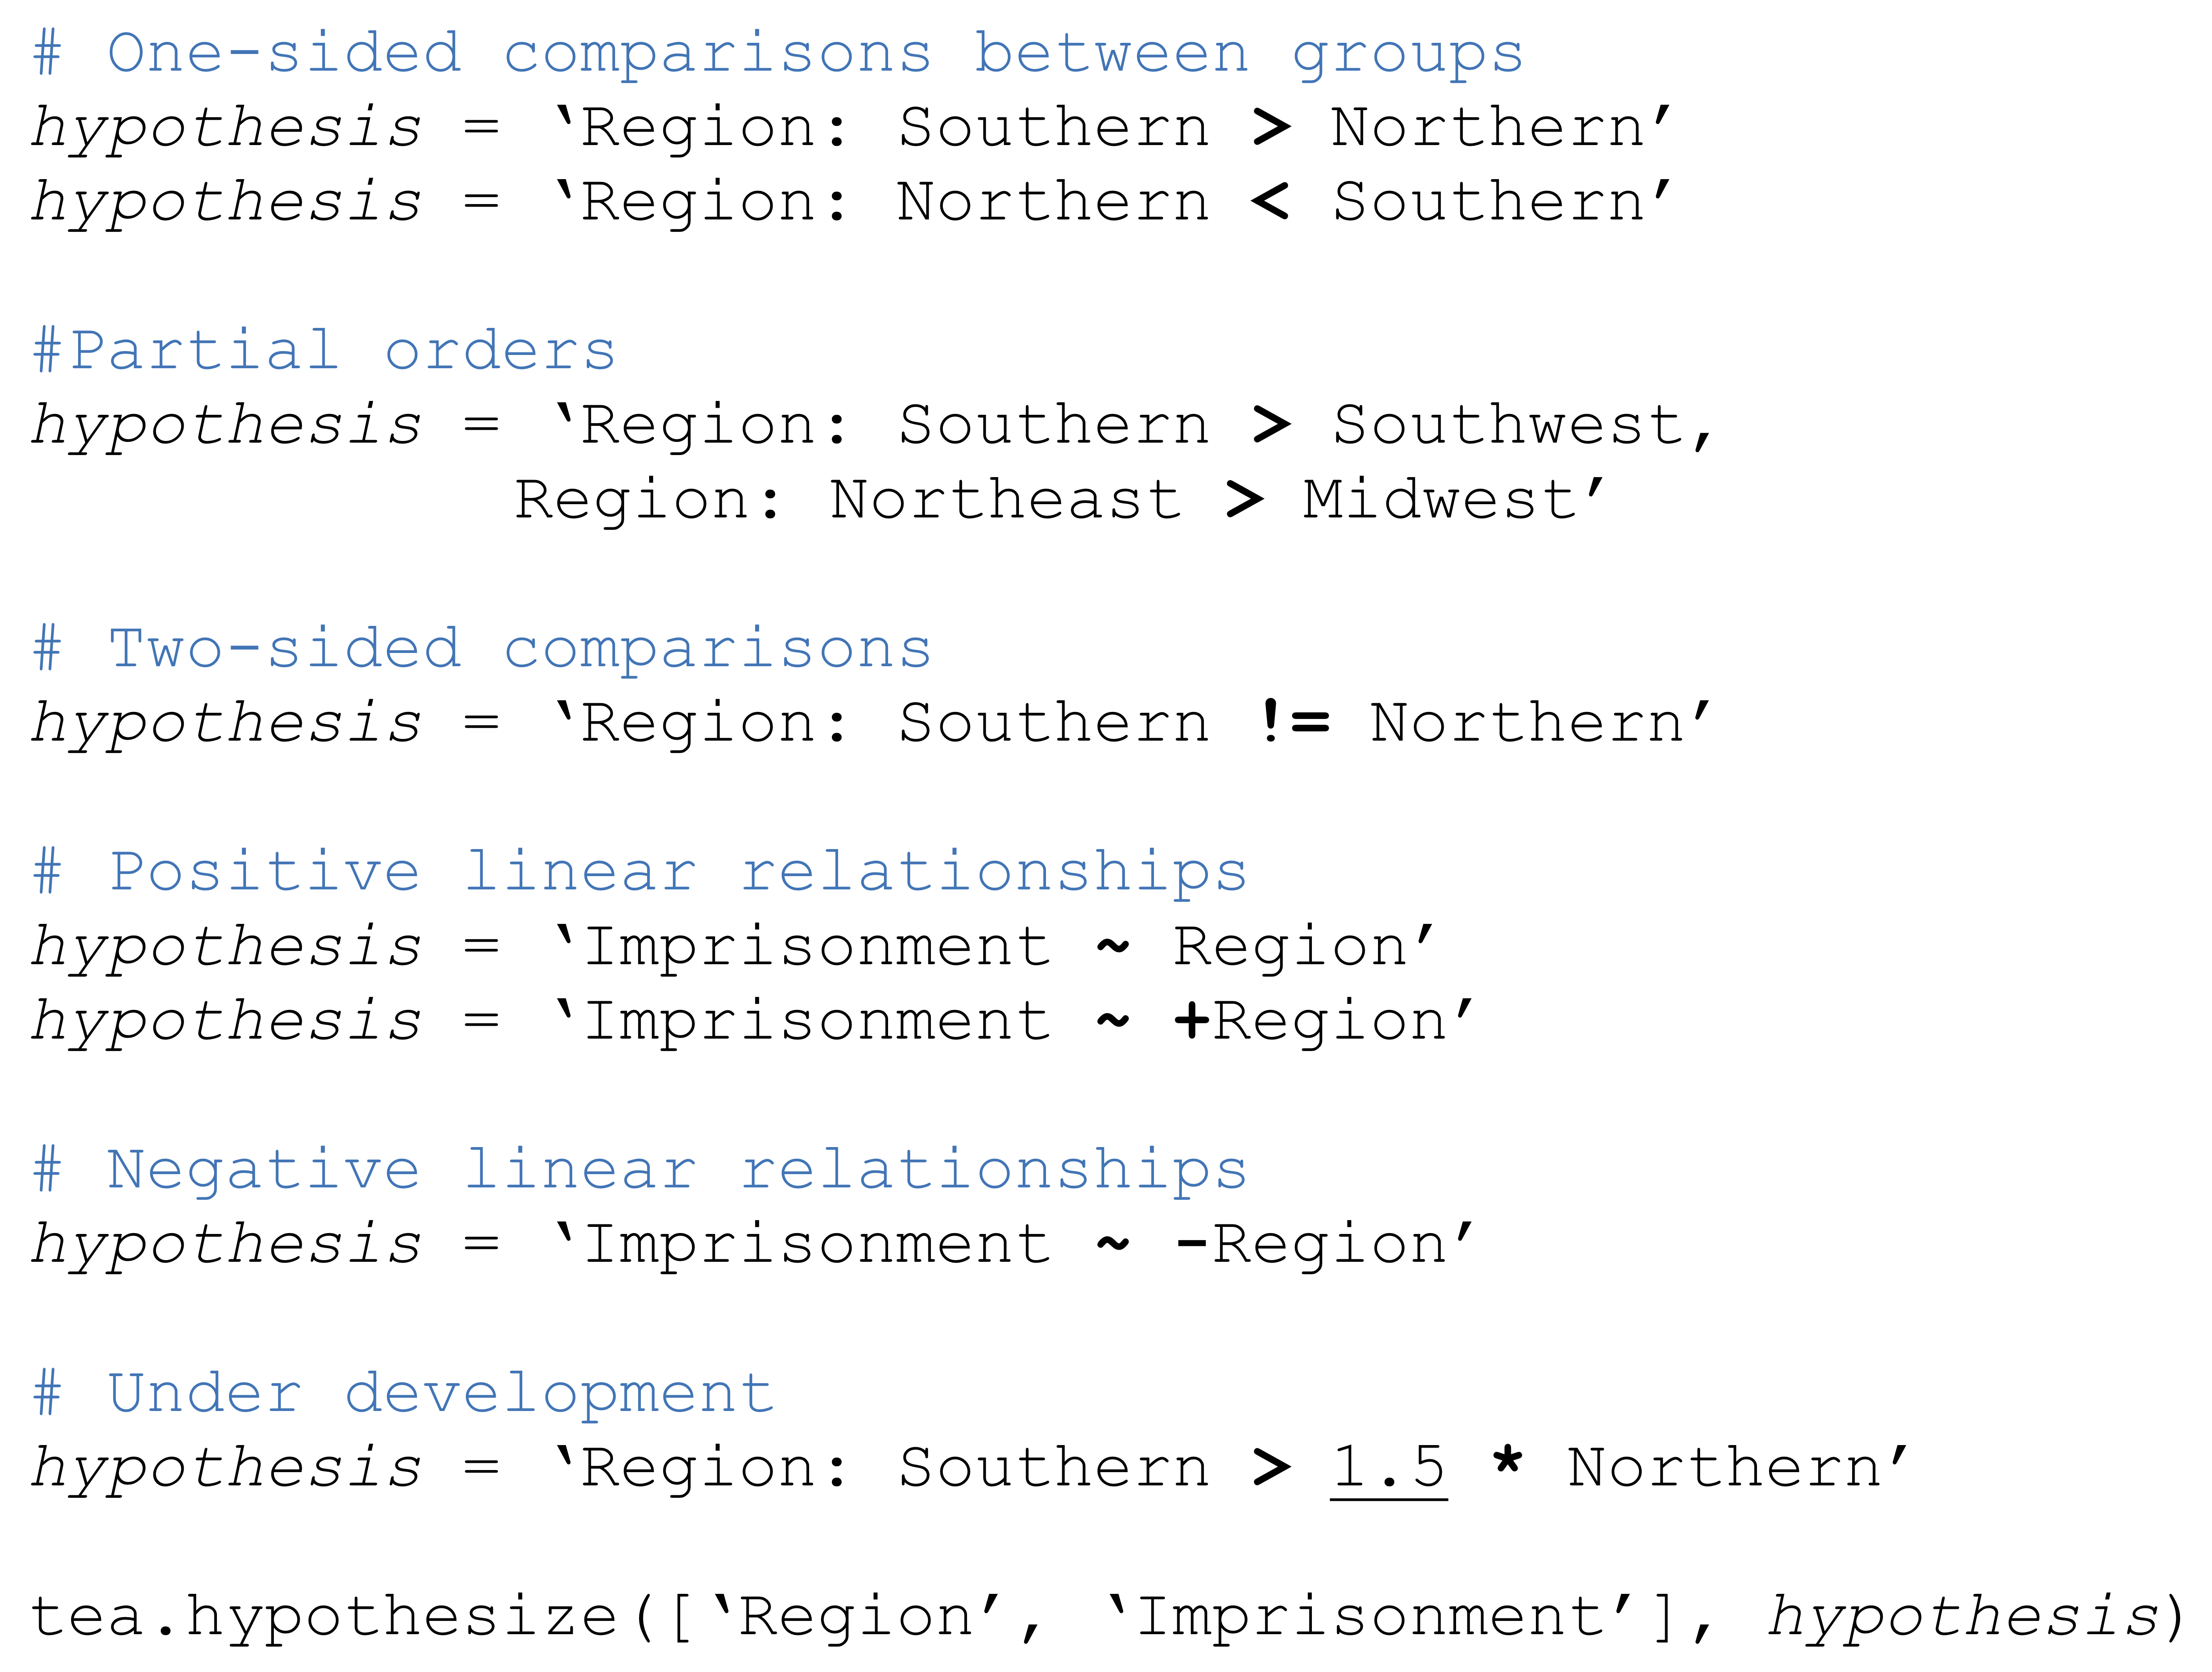
\includegraphics[width=1.\columnwidth, clip]{tea/figures/tea_hypotheses.png}
    % \vspace{-15pt}
    \caption{\textbf{Hypotheses that users can express in Tea.} }
    \label{fig:teaHypotheses}
    \vspace{-\baselineskip}
    \vspace{-3pt}
  \end{figure}
}


\newcommand{\otherSystems}{
    \begin{table*}[t]
        \centering \small
        \caption{\textbf{Comparison of Tea to other tools.} \polish{Format to fit (not run over) horizontally} Despite the published best practices for statistical analyses, most tools do not help users select appropriate tests. Tea not only addresses the best practices but also supports reproducing analyses.}
        \label{tab:otherSystems}
        \begin{tabularx}{\linewidth}{r|c|c|c|c|c|c}
            \colHR{Best practices} & \colH{SAS} & \colH{SPSS} & \colH{JMP} & \colH{R} & \colH{Statsplorer~\cite{wacharamanotham2015statsplorer}} & \colH{Tea} \\
            Explicit statement of user assumptions & \no & \no & \no & \no & \no & \yes \\
            Automatic verification of test preconditions & \no & \no & sometimes & sometimes & \yes & \yes \\
            Automatic accounting of multiple comparisons & \no & \no & \no & \no & \yes & \yes \\
            Surface alternative analyses & \no & \no & \no & \no & \no & \yes \\
            Contextualize results & \yes & sometimes & \yes & sometimes & \yes & \yes \\
            Easy to reproduce analysis & \yes & \yes & \no & \yes & \no & \yes \\
        \end{tabularx}
    \end{table*}
}


\newcommand{\figureOutputTTest}{
  \begin{figure}[t]
    \vspace{-15pt}
    % \centering
    \fbox{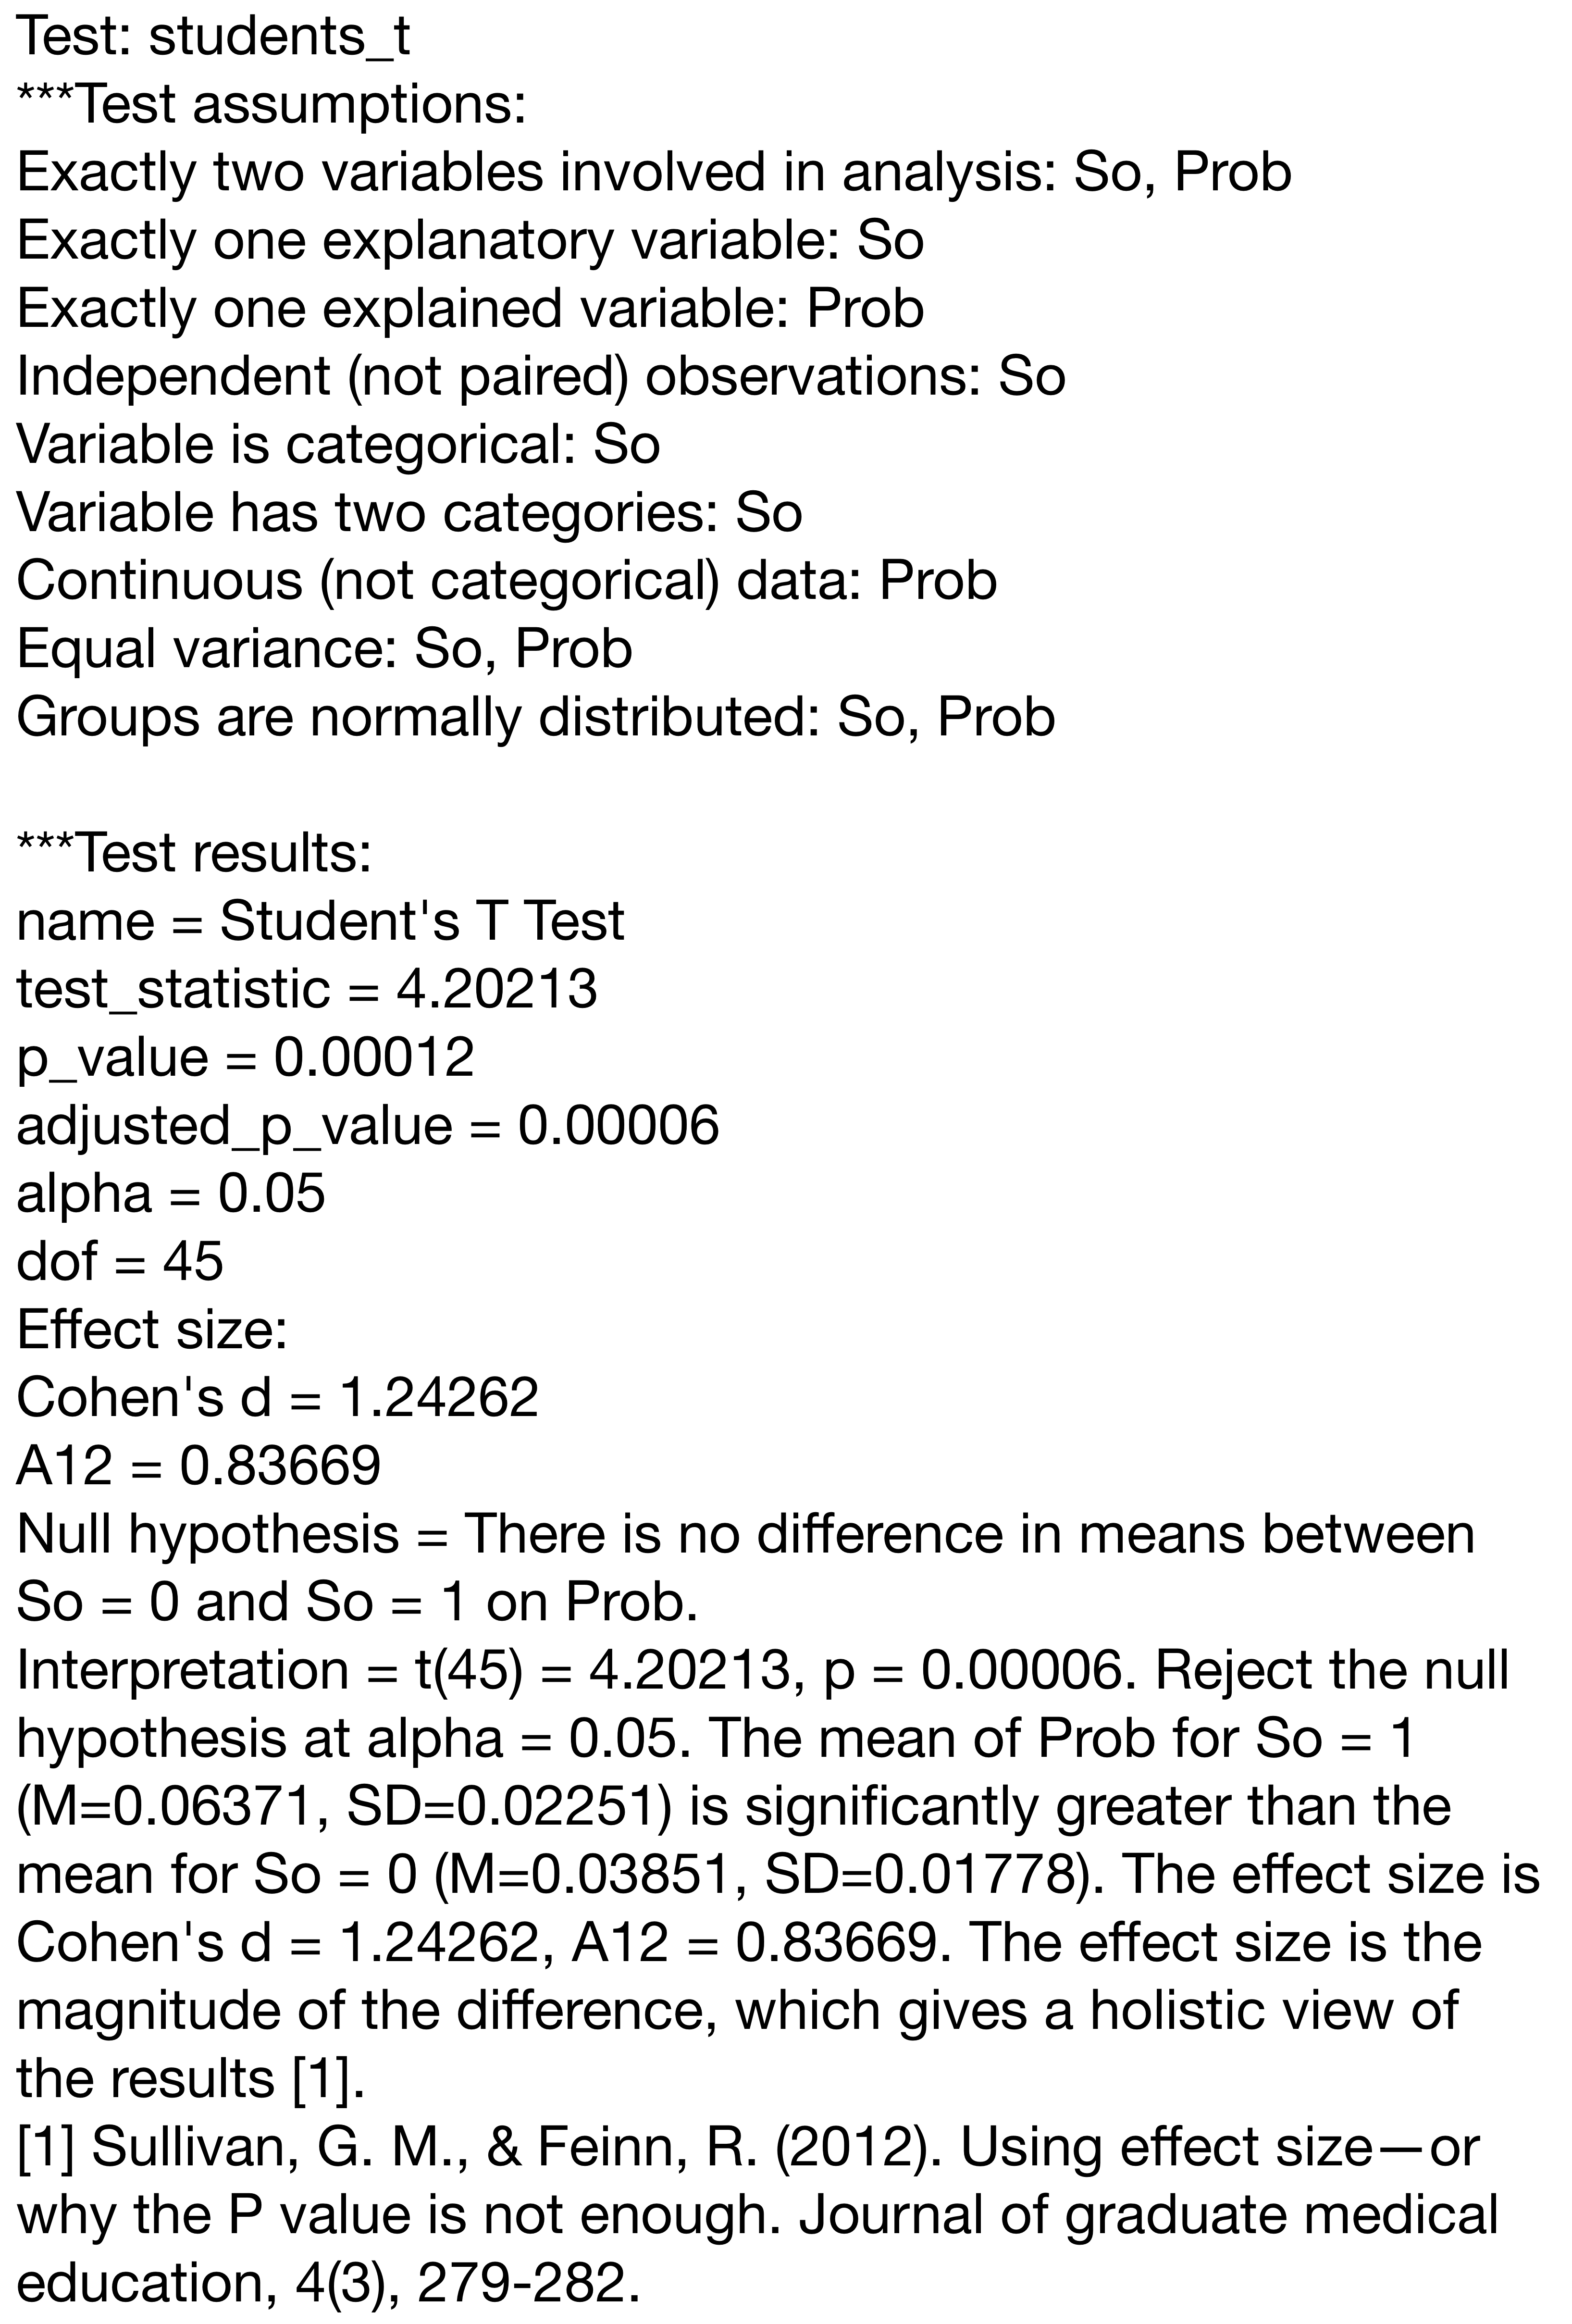
\includegraphics[width=.8\columnwidth, clip]{tea/figures/tea_output_t_test.jpg}}
    \vspace{2pt}
    \caption{\textbf{Part of Tea's output.} The output is a result of running the sample program in Figure~\ref{fig:tea_program}. Tea outputs the data properties that led Tea to select the statistical test as well as results from executing the test, effect size calculations, the null hypothesis tested, and the interpretation of the results, which can be included in publications with minor editing.}
    \label{fig:output_t_test}
    \vspace*{-\baselineskip}
    \vspace{-15pt}
  \end{figure}
}

\newcommand{\figureModes}{
  \begin{figure}[H]
    % \vspace{-5pt}
    \centering
    \includegraphics[width=\textwidth]{tea/figures/modes_wide.jpg}
    \vspace{-10pt}
    \caption{\textbf{Tea program and its mode-dependent executions.} a) Tea program that aims to determine if two contributor variables, `Illiteracy` and `HS Grad' that may predict a third outcome variable `Life Exp', are correlated. The user asserts that `Illiteracy' is normally distributed. 
    b) By default, Tea executes programs in the \textit{strict} mode. 
    c) Warning that Tea disagrees with the user and will override the user's assertion that `Illiteracy' is normally distributed in the \textit{strict} mode. 
    d) Results without the parametric test since Tea overrides user's assertion. 
    e) A single line change can modify Tea to execute a program in \textit{relaxed} mode. 
    f) Warning that Tea cannot verify normality for `Illiteracy' but will defer to user's assertion. 
    g) Results with the parametric test since Tea proceeds as if  `Illiteracy' was normally distributed.}
    \label{fig:modes}
    \vspace*{-\baselineskip}
  \end{figure}
}
 
\newcommand{\figureSyntacticSugar}{
  \begin{figure}
      \centering
      \subcaptionbox{Specify the test.}
      {\fbox{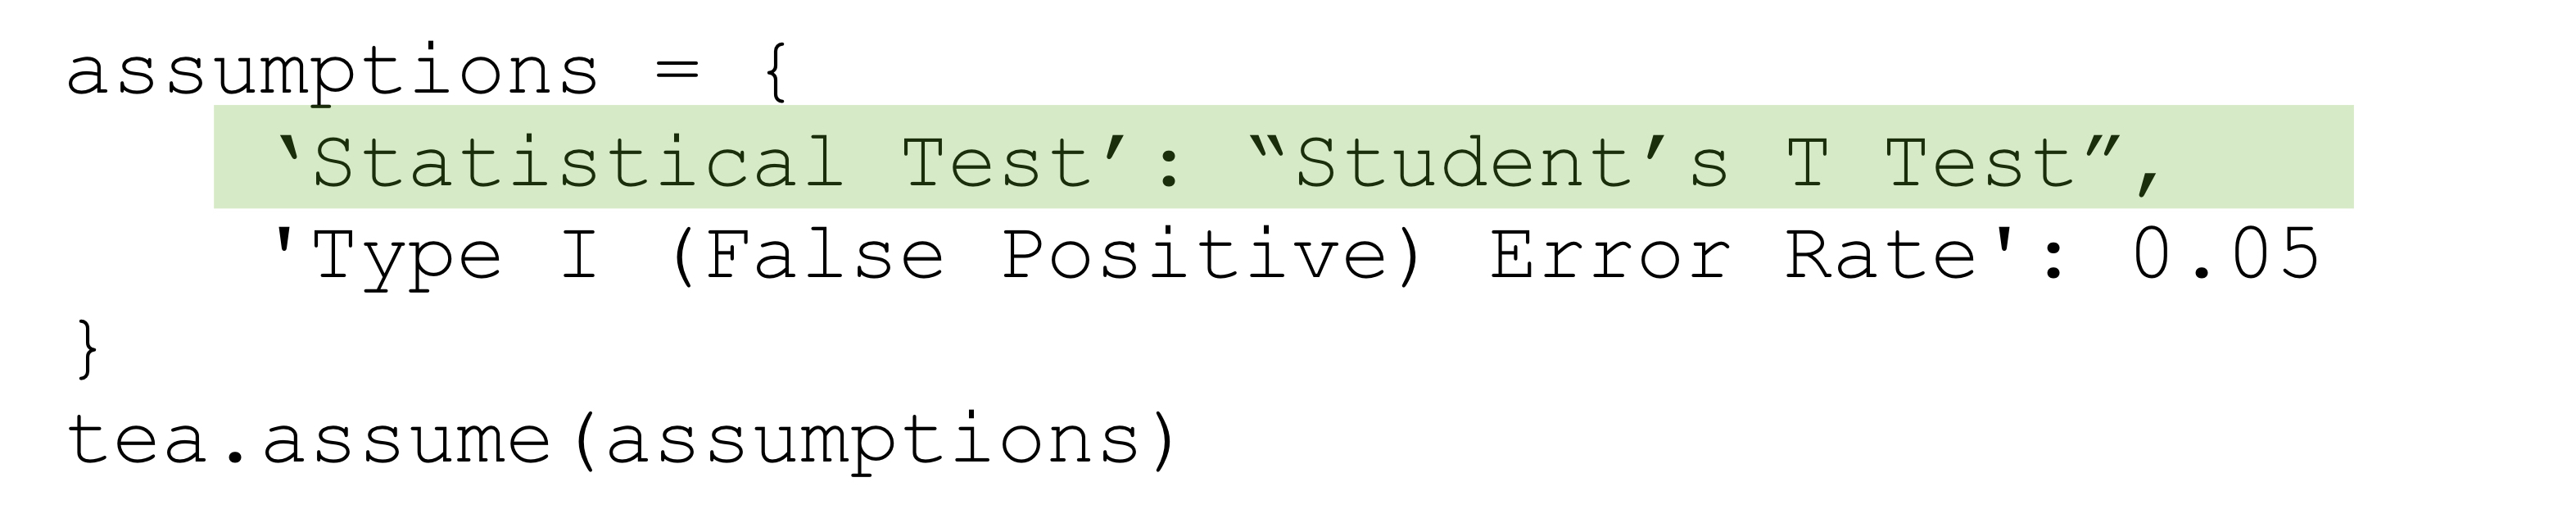
\includegraphics[width=\linewidth, clip]{tea/figures/sugar_test.jpg}}}
      \label{fig:sugar_expanded}
      \subcaptionbox{Specify the properties.}
      {\fbox{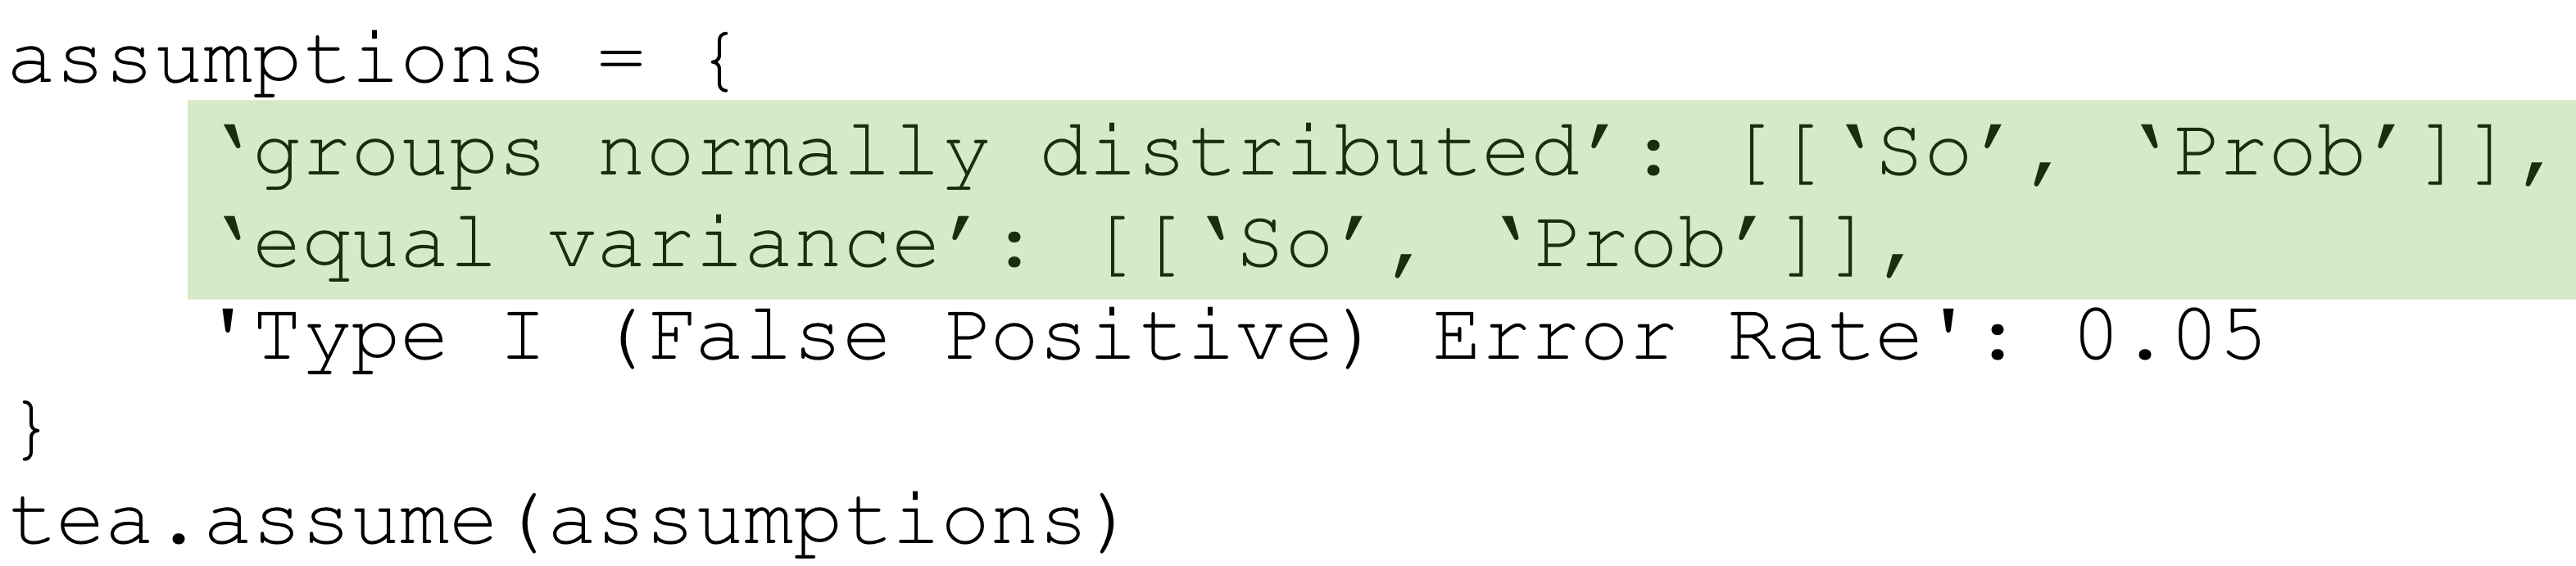
\includegraphics[width=\linewidth, clip]{tea/figures/sugar_expanded.jpg}}}
      \label{fig:sugar_test}
      % \vspace{-10pt}
    \caption{\textbf{Tea can support pre-registration.} Tea programs provide an executable format for pre-registration. When pre-registering studies, users can explicitly state their assumptions about data properties or specify the exact statistical test they intend to run with data. Specifying the name of a test (a) is \textit{syntactic sugar} for the more verbose form (b). The above code snippets are semantically equivalent.}
    \label{fig:sugar}  
    \vspace*{-\baselineskip}
    % \vspace{-3pt}
    \end{figure}
}

\subsection{System overview}
\vspace{-5pt}

Tea consists of a high-level programming language and a runtime system. There
are three key steps to compiling a Tea program from user specifications to
executing statistical analyses:

\begin{enumerate}
    \item \textbf{Check for completeness and syntax.} Tea first checks that a
    user's program specifies a data set, variable declarations, study design
    description, a set of assumptions, and hypotheses using the correct syntax.
    For pre-registration, the
    data set can be empty (with only column names). If there are any syntax
    errors or missing parts, Tea will issue an error and stop execution.
    \item \textbf{Check for consistent, well-formed hypotheses.} Using the
    variable declarations, Tea then checks that the hypotheses the user states
    are consistent with variable data types. For instance, Tea would issue an
    error and halt execution if a nominal variable was hypothesized to have a
    positive relationship with another nominal variable. If the nominal
    variables have categories given by numbers (e.g., a variable for education where `1' stands for `High School', `2'
    for `College', etc. ), a linear relationship would be possible to compute by
    treating the categories as raw continuous values. However, treating the numbers as
    values is incorrect and the results misleading because the numbers represent
    discrete categories, not continuous values. Tea avoids such mistakes.
    \item \textbf{Inspect data properties and infer valid statistical tests.}
    Once Tea's compiler verifies that a Tea program is complete, syntactically
    correct, and consistent, \TeaRS~inspects the data to verify properties
    about it and find a set of valid statistical tests. The
    higher-level Tea program is then compiled to logical constraints, which is
    further discussed in~\autoref{sec:TeaRS}.
\end{enumerate}

\vspace{-5pt}
\subsection{Tea's Domain-Specific Programming Language} \label{sec:TeaPL}
% \figureOutputTTest
Tea is a domain-specific language
embedded in Python. It takes advantage of existing Python data structures (e.g.,
classes, dictionaries, and enums). We chose Python because of its widespread
adoption in data science. Tea is itself implemented as a Python library\footnote{Tea is open-source and available for download on
\texttt{pip}, a common Python package manager.}.

A key challenge in describing studies is determining the level of granularity
necessary to produce an accurate analysis.  In Tea programs, users describe
their studies in five ways: (1) providing a data set, (2) describing the
variables of interest in that \dataSet, (3) specifying their study design, (4)
stating their assumptions about the variables, and (5) formulating hypotheses
about the relationships between variables. Figure~\ref{fig:modes} shows an
an exaample Tea program and its output. 


\subsubsection{Data}
Data is required for executing statistical analyses. One challenge in managing
data for analysis is minimizing both duplicated data and user intervention.

To reduce the need for user intervention for data manipulation, Tea
requires the data to be a CSV in long format. CSVs are a common output
format for data storage and cleaning tools. Long format (sometimes
called ``tidy data''~\cite{wickham2014tidy}) is a denormalized format
that is widely used for collecting and storing data, especially for
within-subjects studies.

Unlike R and Python libraries such as numpy~\cite{oliphant2006numpy}, Tea only
requires one instance of the data. Users do not have to duplicate the data or
subsets of it for analyses that require the data to be in slightly different
forms. Minimizing data duplication or segmentation is also important to avoid
user confusion about where some data exist or which subsets of data pertain to
specific statistical tests.

Optionally, users can also indicate a column in the \dataSet that acts
as a relational (or primary) key, or an attribute that uniquely
identifies rows of data. For example, this key could be a participant
identification number in a behavioral experiment. A key is useful for
verifying a study design, described below. Without a key, Tea's default
is that all rows in the data set comprise independent observations (that is, all
variables are between subjects).

For pre-registration where there is no data, a CSV with only column names is necessary.

\vspace{-7pt}
\subsubsection{Variables}
Variables represent columns of interest in the data set. Variables
have a name, a data type (\emph{nominal}, \emph{ordinal},
\emph{interval}, or \emph{ratio}), and, when appropriate, valid
categories.  Users (naturally) refer to variables through a Tea program using
their names. Only nominal and ordinal variables have a list of
possible categories. For ordinal variables, the categories are also
ordered from left to right.

Variables encapsulate queries. The queries represent the index of the
variable's column in the original data set and any filtering
operations applied to the variable. For instance, it is common to
filter by category for nominal variables.
% in statistical tests.

\vspace{-7pt}
\subsubsection{Study Design}
Three aspects of study design are important for conducting statistical
analyses: (1) the type of study (observational study vs. randomized
experiment), (2) the independent and dependent variables, and (3) the
number of observations per participant (e.g., between-subjects
variables vs. within-subjects variables).

For semantic precision, Tea uses different terms for independent and
dependent variables for observational studies and experiments.  In
experiments, variables are described as either ``independent'' or
``dependent'' variables. In observational studies, variables are either
``contributor'' (independent) or ``outcome'' (dependent) variables. 
% If variables are neither independent nor dependent, they are treated as co-variates.

\vspace{-7pt}
\subsubsection{Assumptions} \label{subsec:assumptions}
Users' assumptions based on domain knowledge are critical for
conducting and contextualizing studies and analyses. Often, users'
assumptions are particular to variables and specific properties (e.g.,
equal variances across different groups). Current tools generally do
not require that users encode these assumptions, leaving them implicit.

Tea takes the opposite approach to contextualize and increase the
transparency of analyses. It requires that users be explicit about
assumptions and statistical properties pertaining to the analysis as a
whole (e.g., acceptable Type I error rate/significance threshold) and
the data.


Tea supports two modes for treating user assumptions: \textit{strict} and
\textit{relaxed}. In both modes, Tea verifies all user assumptions and issues
warnings for assumptions that statistical testing does not verify. In the
\textit{strict} mode, Tea overrides user assumptions when selecting valid
statistical tests. In the \textit{relaxed} mode, Tea defers to user assumptions
and proceeds as if the assumptions verified even if they did not. The
\textit{strict} mode is the default, but users can specify the \textit{relaxed}
mode. Figure~\ref{fig:modes} shows the two modes and the different warnings and
output they generate.
\figureModes

If users also know that a data transformation (i.e., log transformation) applies
to a variable, they can express this as an assumption. Data transformations are
not properties to be verified but rather treatments of data that are applied
during assumption verification, statistical test selection, and test execution,
which is why they are included in the assumptions clause. The next section discusses the
verification process for assumptions in greater detail.


\vspace{-7pt}
\subsubsection{Hypotheses}
% \teaHypotheses
Hypotheses drive the statistical analysis process. Users often have
hypotheses that are technically alternative hypotheses.

Tea focuses on capturing users' alternative hypotheses about the
relationship between two or more variables. Tea uses the alternate
hypothesis to conduct either a two-sided or one-sided statistical
test. By default, Tea uses the null hypothesis that there is no
relationship between variables.

% \todo{Add table of hypotheses}

% Figure~\ref{fig:teaHypotheses} exemplifies the range of hypotheses Tea supports.

\subsection{Tea's Runtime System} \label{sec:TeaRS}
Tea compiles programs into logical constraints about the data and
variables, which it resolves using a constraint solver. A significant
benefit of using a constraint solver is extensibility. Adding new
statistical tests does not require modifying the core of Tea's runtime
system. Instead, defining a new test requires expressing a single new
logical relationship between a test and its preconditions.

At runtime, Tea invokes a solver that operates on the logical
constraints it computes to produce a list of valid statistical tests
to conduct. This process presents three key technical challenges: (1)
incorporating statistical knowledge as constraints, (2) expressing
user assumptions as constraints, and (3) recursively selecting
statistical tests to verify preconditions of other statistical tests.

\vspace{-3pt}
\subsubsection{SMT Solver}
As its constraint solver, Tea uses Z3~\cite{de2008z3}, a Satisfiability Modulo Theory (SMT) solver.

Satisfiability is the process of finding an assignment to variables that makes a
logical formula true. For example, given the logical rules $0 < x < 100$ and $y
< x$, \{$x = 1, y = 0$\}, \{$x = 10, y = 5$\}, and \{$x = 99, y = -100$\} would all be
valid assignments that satisfy the rules. SMT solvers determine the
satisfiability of logical formulas, which can encode boolean, integer, real
number, and uninterpreted function constraints over variables. SMT solvers can also
be used to encode constraint systems, as we use them here. A wide variety of 
applications ranging from the synthesis of novel interface
designs~\cite{swearngin2018scout}, the verification of website
accessibility~\cite{panchekha2018verifying}, and the synthesis of data
structures~\cite{loncaric2016cozy} employ SMT solvers. 

\vspace{-7pt}
\subsubsection{Logical Encodings}
The first challenge of framing statistical test selection as a constraint satisfaction
problem is defining a logical formulation of statistical
knowledge.

Tea encodes the applicability of a statistical test based on its preconditions.
A statistical test is applicable if and only if all of its preconditions (which
are properties about variables) hold. We derived preconditions for tests
from an online HCI and statistics course~\cite{klemmerCoursera}, a statistics
textbook~\cite{field2012discoveringR}, and publicly available data science
resources from universities~\cite{ucla:whatstat, kent:tutorials}.

Tea represents each precondition for a statistical test as an uninterpreted
function representing a property over one or more variables. Each property is
assigned \texttt{true} if the property holds for the variable/s; similarly, if the
property does not hold, the property function is assigned \texttt{false}.

Tea also encodes statistical knowledge about variable types and properties that
are essential to statistical analysis as axioms, such as the constraint that only a
continuous variable can be normally distributed.

\vspace{-10pt}
\subsubsection{Algorithm}
Tea frames the problem of finding a set of valid statistical tests as a maximum
satisfiability (MaxSAT) problem that is seeded with user assumptions.

First, Tea translates each user assumption about a data property into an axiom
about a property and variable. As described in~\autoref{subsec:assumptions}, user
assumptions about properties but not data transformations are always checked. In
the \textit{strict} mode, Tea overrides any user assumptions it does not find to
hold, creating an axiom that a property is \texttt{false}. In the \textit{relaxed} mode, Tea
    defers to user assumptions, creating axioms that a property is \texttt{true}. For
any user assumptions that do not pass statistical testing, Tea warns the user and explains
how it will proceed depending on the mode.

Then, for each new statistical test Tea tries to satisfy, Tea checks to see if
each precondition holds. For each precondition checked, Tea adds the property
and variable checked as an axiom to observe as future tests are checked. If any
property violates the axioms derived from users' assumptions, the property is
removed and the test is invalidated. Users' assumptions
always take precedence.


The constraint solver then prunes the search space. Tea does not compute all
properties for all variables, a significant optimization when
analyzing very large data sets.

At the end of this process, Tea finds a set of valid statistical tests
to execute. If this set is empty, Tea defaults to its implementation
of bootstrapping~\cite{efron1992bootstrap}. Otherwise, Tea proceeds
and executes all valid statistical tests. Tea returns a table of
results to users, applying multiple comparison corrections~\cite{holm1979simple} and
calculating effect sizes when appropriate.

\vspace{-10pt}
\subsubsection{Optimization: Recursive Queries}
When Tea verifies a property holds for a variable, it often must invoke another
statistical test. For example, to check that two groups have equal variance,
Tea must execute Levene's test. The statistical test used for
verification may then itself have a precondition, such as a minimum sample size.

Such recursive queries are inefficient for SMT solvers like Z3 to reason
about. To eliminate recursion, Tea lifts some statistical tests to properties.
For instance, Tea does not encode the Levene's test as a statistical test.
Instead, Tea encodes the property of having equal variance between groups and
executes the Levene's test for two groups when verifying that property for particular variables.
\vspace{-3pt}

\vspace{-2pt}
\subsubsection{User Output}
The result of running a Tea program with data is a listing of the results of
executing valid statistical tests, as shown in Figure~\ref{fig:modes}. For each valid
statistical test executed, the output contains the properties of data that Tea
checked and used to determine that a statistical test applied, the test
statistic value, p-value (and an adjusted p-value, if applicable), effect sizes
(Cohen's $d$~\cite{cohen1988statistical} and Vargha Delaney
A12~\cite{vargha2000critique}), the alpha level the user specified in their
program, the precise null hypothesis the statistical test examined, an
interpretation of the results in APA format~\cite{american1983publication}, and text
recommending users to focus on effect size rather than the p-value for a
holistic view of their data. This output is intended to inform users of why Tea
selected specific statistical tests and how to interpret their results.

% \todo{This output is continuing to change and be updated to incorporate visualizations to give users more context and helpfufl outputs for inclusion in future manuscripts.}
